\documentclass[twocolumn,11pt,english]{article}
\usepackage{listings}
\usepackage{amsmath}
\usepackage{amsfonts}
\usepackage{cite}
\usepackage[T1]{fontenc}
\usepackage{graphicx}
\usepackage{color}
\usepackage[margin=1.0in]{geometry}
\lstset{language=Haskell}

\addtolength{\topmargin}{-0.5in}

\title{Maybe Slipstreams}
\date{}
\author{
  Carlyle, John\\
  \textit{jcarlyle@ucsc.edu}
  \and
  McDermott, Morgan\\
  \textit{mmcdermo@ucsc.edu}
}


\begin{document}
\maketitle

\section{Abstract}
We give a definition of \textit{Functional Reactive Programming} (FRP) that allows for dynamic signal networks and safe interaction with the real world. We allow signal networks to be dynamic by modeling them as higher-order streams (as in Patai \cite{HighOrderStreams}), and use the concept of wormholes (from Winograd \cite{WinogradCort2012HS}) to make interaction with real world resources safe. All signal values are modeled as $Maybe$ values to allow for defined behavior in the face of disrupted signals, and to reference signal values before they have any reasonable value. We also specify a DSL that uses this FRP model, allowing a programmer to easily design signal networks to accomplish tasks by specifying layers and how the layers interact. Our implementation builds on previous work by being more practical. The DSL arises naturally from our definition of FRP, is simple to use and requires only limited knowledge of the underlying FRP concepts.

\section{Introduction}
  
\subsection{What is FRP}
Functional Reactive Programming, introduced by Fran \cite{ElliottHudak97:Fran}, is a programming paradigm based on time varying values. The fundamental idea behind it is to allow the programmer to express than ``what'' of a program, and the ``how'' of the program be infered. FRP operates by a series of \textit{behaviors}, which are time varying values that react with one another to form a program. 

\subsection{Why use FRP}
FRP is a useful approach to user interface design because it is declarative. Most interface design forces you to define exactly how to generate each value and once the value is generated. The common approach leads to extremly messy interface code. With the time varying values supplied by an FRP network the programmer can choose \textit{what} an interface element is rather than how it is generated. By comosing these values together a higher-level description of what each interface element should be. From this declarative structure the relationship between pieces of the interface implicitly emerges, freeing the programmer from having to tediously define exactly how each relationship is enacted.

\subsection{Problems with FRP}
We solve the problem of interacting with time-varying values using stream-based FRP, where each computation sends a stream instead of a signal value. A stream is essentially a complete history of the values of a particular computation. Any other computation that needs the current value, or a value from the past, can look at the stream and find the appropriate values. This leads to additional problems like memory usage growing out of control as new values are continually added to the stream and not removed. In some systems garbage collection finds and removes values from streams that are no longer dependencies for other computations. In Elerea \cite{HighOrderStreams}, this is solved by only allowing access to the most recent values in streams. 


\subsection{Organization}
This paper primarily introduces a way for FRP to interact safely in an environment filled with hazerdous resources which are difficult to model as a function of time. (What the different sections are for) (Section 1) Section 2 Section 3 Section 4 Section 5 Section 6 Section 7.

\section{A Motivating Example}
Adapting FRP for javascript development would be super fantastic since javascript GUI code deals with varying values all the time. In particular the asynchronous communication between a server and client through the use of AJAX can be thought of as a time-varying signal between two nodes. 

There are several problems that must be solved in stream-based FRP to allow this transaction to take place. First, how do we interact with the environment itself? Since we need to manipulate the DOM and perform asynchronous requests, we have to change state. 

Secondly, how do we model the changing requirements for interfaces? If the user presses a button to submit a query to the server, the server could respond in a way indicating that they need to update the interface on the page. Perhaps we need to create more buttons that could perform different server queries. In order to solve this, we must define a flexible, dynamic FRP network that can modify itself. Elerea solves this by providing Higher-Order Streams. 

We need to ensure that the time-based values from the server are treated in a well-defined way. Namely, what if we have never contacted the server? What should the value of its stream be, and how should that differ from the stream after it has responded and is in an idle state again? We solve this by encapsulating every stream value in a $Maybe$, as we will explain later. 

Lastly, what happens when two computations wish to change the state of the interface at the same time? How can we allow safe interaction between external state and multiple FRP calculations that wish to modify the state? We solve this using Wormholes as defined by Winograd-Cort \cite{WinogradCort2012HS}.

\section{FRP Terminology}

\begin{description}


\item[behavior] Using the previous definition of an element and a signal, an element can be thought of as a function that maps from one signal to another. More concretely \\
  $type~element~a~b = Signal ~a \rightarrow Signal ~b$\\
  Behaviors are typically thought of in terms of continuous functions. What FRP is trying to do is model the change in behavior of some element in a network. This takes up a lot of processor power  and is not very efficient.

\item[event] An event is a discrete behavior. Since behaviors perform so poorly, it is often necessary to break a signal into a set of discrete values. The cutoff is not clear between high and low sampling rates. With a high sample rate, something can be considered a behavior; with a low sample rate it can be considered an event. Our implementation of FRP is skewed toward events.

\item[signal] It is useful to think of the values being sent from one element to another as a signal being broadcast continuously. The element receiving this signal adjusts its own outgoing signal according to a predefined set of rules or a function.

\item[stream] An element may have need of signals from more than one timestep in the past. A stream is essentially a history of all previous values of a signal, with the most current signal value at the head of the list. Streams travel between elements, thus allowing an element to select what timestep it selects a value from. The downside of streams is that they allow for spacetime leaks, which are described below. A stream of type $Stream~a$ will be denoted as $\langle v_0~v_1~v_2~...\rangle$ where $v_i$ is of type $
a$.

\item[space-time leak] In a functional reactive service, any particular element can depend on values that are far in the past. Clearly, the longer the program is executing, the longer the history of events, or the longer the stream is. A longer stream takes up more memory and can cause slowdown if the stream is not trimmed after a certain point. Typically a garbage collection service of some kind is used to clean up old events upon which are no longer being depended.. This is analogous to a memory leak in imperative programming. The value is said to be a space-time leak if it is unnecessarily being used for computations when it will have no effect on any current elements.
\end{description}

\section{Network Dynamism through Higher Order Streams}
In order to express the dynamic behavior that we need to implement GUIs, the underlying signal network needs to be able to change itself over time. We choose to model this dynamism with higher order streams like Patai\cite{HighOrderStreams}. This method avoids the time and space leaks that were present in other FRP systems with first class signals/behaviors/events \cite{ElliottHudak97:Fran}. 

Patai defines his model in terms of \textit{Denotational Design} developed by Conal Elliot \cite{elliott2009denotational}. The core idea Patai leverages is the \textit{Type Class Morphism}, or defining an interface by a combination of its \textit{type} and its \textit{properties}. By focusing on the interface, this design strategy allows implementations to be checked for correctness but to otherwise have freedom in their methodology. 

The core type in Patai's stream model is \textit{Stream a}, representing a stream of values over time. This is analagous to a Behavior, and in fact has the same type signature: 
\begin{equation}
  \textbf{type}~\textit{Stream a} = \mathbb{N} \rightarrow a
\end{equation}
Any  s::\textit{Stream a} can be thought of as the stream of values:
\begin{equation}
  \langle s_0 s_1 s_2 ... s_n \rangle ~where~ s_i :: a
\end{equation}
Initially Patai models these Streams using a \textit{cons} constructor that represents a delay of one timestep. However, if we use this stream definition and consider a higher order stream of type \textit{Stream (Stream a)}, we end up with quadratic performance for \textit{join} when we attempt to extract a value from the \textit{Stream (Stream a)}. This is fairly obvious if we try to visualize the higher order stream, since the values of $join~s$ where $s$ :: \textit{Stream (Stream a)} are the main diagonal of the stream of streams:

\begin{align*}
    \langle &\langle \mathbf{v_{00}} ~ v_{01} ~ v_{02} ~ ... ~ \rangle \\
    &\langle v_{10} ~ \mathbf{v_{11}} ~ v_{12} ~ ... ~ \rangle \\
    &\langle v_{20} ~ v_{21} ~ \mathbf{v_{22}} ~  ...  ~ \rangle \rangle
\end{align*}

To solve this problem, Patai moves away from the \textit{cons} definition of Streams. Instead, he creates streams and higher order streams from three primitives: $delay$, $start$, and $generator$. He also introduces the type $StreamGen$, which has the same signature as a $Stream$ but is only used to represent higher order streams. 

\small
\begin{equation}
  \mathbf{type}~\mathit{StreamGen~a} = \mathbb{N} \rightarrow a
\end{equation}
\normalsize
The $delay$ function replaces cons in this new configuration. The difference is that instead of returning a $Stream$, it returns a $StreamGen$. It functions by returning its first argument at $t = 0$, and the first $Stream~a$ applied to the sample time otherwise. For intuition, we've also included the simplified type:
\small
\begin{align*}
dela&y :: a \rightarrow Stream~a \rightarrow StreamGen~(Stream~a)\\
dela&y :: a \rightarrow (\mathbb{N} \rightarrow a) \rightarrow (\mathbb{N} \rightarrow~(\mathbb{N} \rightarrow~a))\\
dela&y~x~s~t_{start}~t_{sample} =\\
&|~t_{start} = t_{sample} = x\\
&|~t_{start} < t_{sample} = s (t_{sample} - 1)\\
&|~otherwise ~~~~~~=\perp
\end{align*}
\normalsize

The $start$ function simply gives us a safe way to extract a stream from a stream generator. Given that $delay$ is undefined if $t_{start} > t_{sample}$, a universally safe time for $t_{start}$ is 0.
\small
\begin{align*}
&start :: StreamGen (Stream~a) \rightarrow Stream a\\
&start g = g~0
\end{align*}
\normalsize

However, given $t_{sample}$ there is another safe value: $t_{start} = t_{sample}$. This concept is embodied in the function $generator$: 
\small
\begin{align*}
&generator :: Stream~ (StreamGen a) \rightarrow Stream~a\\
&generator~g~t_{sample} = g~t_{sample}~t_{sample}
\end{align*}
\normalsize


TODO: DISCUSS THE FANCY EFFICIENCIES AND BIND AND JOIN ETC
\begin{align*}
  \langle &\langle \mathbf{v_{00}} ~ v_{01} ~ v_{02} ~ v_{03} ~ ... ~ \rangle \\
  &\langle \perp ~ \mathbf{v_{11}} ~ v_{12} ~ v_{13} ~... ~ \rangle \\
  &\langle \perp ~ \perp ~ \mathbf{v_{22}} ~ v_{23} ~ ...  ~ \rangle \rangle
\end{align*}


Better idea to avoid wasted space and complex ge


\begin{align*}
  \langle &\langle \mathbf{v_{00}} ~ v_{01} ~ v_{02} ~ v_{03} ~ ... ~ \rangle \\
  &\langle  \mathbf{v_{11}} ~ v_{12} ~ v_{13} ~ v_{14} ~ ... ~ \rangle \\
  &\langle  \mathbf{v_{22}} ~ v_{23} ~ v_{24} ~ v_{25} ~ ...  ~ \rangle \rangle
\end{align*}


\section{Real World Interfaces}
\subsection{Signals as Maybe Streams}
  Consider modeling a stream of data from a server to a browser GUI. There are two situations when the value of this stream might have an undefined value: If the connection between server and browser has not yet been initiated, or if it has been disrupted. 

To model the two cases of \textit{disruption} and \textit{pre-existence}, we introduce what we call a $Signal$, which is roughly modeled as:
\begin{equation}
  \textbf{type}~\textit{Signal a} = Stream (Maybe~a)
\end{equation}

At any point in time, a $Signal$ may now be defined but have a $Nothing$ value. We can now be assured that any system behavior dependent on this value will act in a defined way even given possible disruption. 

As in the given motivating example, we could now also reference the current value of a stream of data coming from the server before we ever initiate the connection.

\subsection{Wormholes}
\cite{WinogradCort2012HS}

\section{DSL}

A major roadblock in FRP adoption is its complexity. Understandably, FRP implementations attempt to be as expressive as possible. Our implementation, for example, extended the basic idea of Elerea and Elm with additional safety measures for real world interaction. 

The goal of our DSL is to bridge the gap between a complex, fully expressive FRP system, and something that can be easily used to express a usable FRP program. It is intended to rest atop more complicated FRP libraries, enabling access for a new class of end users who want a quick and intuitive interface.

\subsection{DSL Components}

When implementing software with FRP, dependencies between values can be confusing. This is why in our DSL, we restrict dependencies by dividing Signal values into \textit{layers}. Layers are composed of \textit{elements}, representing time-varying values ($Signal$s) computed from previous values. To maintain the desired ease of understanding, elements can only depend on the values of elements from the previous layer. 

\begin{figure}[h!]
  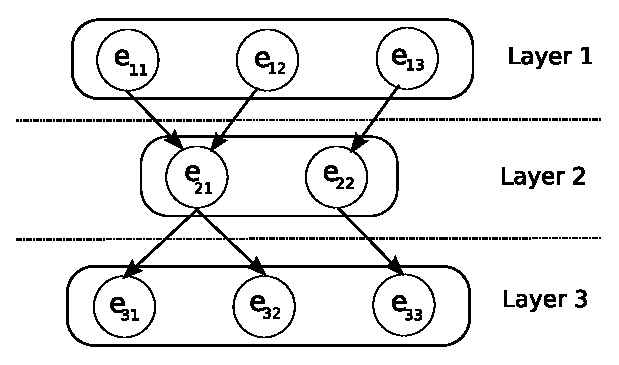
\includegraphics[scale=0.8]{layers.eps}
\caption{DSL Layers and Elements}
\label{fig:layers}
\end{figure}

In Figure~\ref{fig:layers}, arrows represent dependencies. Element $e_{22}$, for example, depends on $e_{11}$ and $e_{12}$. In this system, the output of the FRP program is defined as the tuple of the values of the elements of the last layer; The output of this FRP program would be $(e_{31}, e_{32}, e_{33})$.

\subsection{DSL Definitions}
\begin{description}
\item[element] Any time-varying value, or any computation that relies upon previous computations or values. An element is essentially a Signal Function that has arity from 0 to $n$ where $n$ is the size of the previous layer. All elements connected to element $e$ can be split into two sets: $s_1$ (all elements supplying input to $e$) and $s_2$ (all elements recieving their input from $e$). $s_1$ is called the predecessor set of $e$ or $s_1 = pred(e)$, and $s_2$ is the successor set of $e$ or $s_2 = succ(e)$

\item[network] A set of elements that form a connected component. Multiple networks can be used to describe different unrelated components of a particular interface or problem space.

\item[layer] A layer is a set of elements in a network where the intersection of their mutual union of predecessor and successor sets is the empty set. More formally,
\begin{equation}
  \bigcup_{e_i \in L}{pred(e_i)} \cap \bigcup_{e_j \in L}{succ(e_j)} = \emptyset
\end{equation}
where $L$ is a layer. Breaking a network into layers is helpful because it helps identify dependencies in the network. It also helps introduce structure into the environment, which can help organize a network during its development. 
\end{description}
The DSL defined in this way cannot express many network topologies. For example, it cannot express feedback loops, and has no way of passing a result back to a predecessor. This technique is useful for maintaining state in a network, and there are many other practical uses for it. 

\subsection{DSL Examples}
The goal of the DSL is to easily express \textit{networks} as we've defined them. To express the network from Figure~\ref{fig:layers}, we would write:
\begin{center}
$(e_{11}, e_{12}, e_{13})$
\\ $\rightarrow (e_{21}, e_{22})$
\\ $\rightarrow (e_{31}, e_{32}, e_{33})$
\end{center}
The elements in layer 1 represent functions of type $() \rightarrow Signal~a$, while the elements in all other layers represent a signal function of any arity, i.e.) $Signal~(a, b, ... n) \rightarrow Signal~z$

A program in the actual DSL would therefore have $source$s in the first layer and signal functions or sources elsewhere. Builtin functions of type $() \rightarrow Signal~a$ are prefixed by $@$ in our DSL for clarity. 

In our DSL, $L[expr]$ represents the lifting of an anonymous function that takes as arguments the values of all elements in the previous layer, and whose body is $expr$. That is, 
\begin{center}
$L[\$1 * \$2] \equiv lift (\backslash \$1 ~\$2 \rightarrow \$1 * \$2)$
\end{center}
Using these constructs, a specific network with the same topology as Figure~\ref{fig:layers} might be:
\begin{center}
$(@mousePosX, @mousePosY, @time)$
\\ $\rightarrow (L[sum(\$1, \$2)], L[\$3 * 2])$
\\ $\rightarrow (L[\$1 / 2], L[\$1], L[\$3])$
\end{center}
\subsection{DSL Grammar}
\footnotesize
\begin{align*}
  Statement ::=& ~V \leftarrow Expression &\text{Variable assignment}\\
  |& ~Expression &\text{Single expression}\\
  Expression ::=& ~SignalNet &\text{A signal network}\\
  |& SimpleExpr &\text{An expression}\\
  SignalNet ::=& ~( Exprs ) \rightarrow SignalNet &\text{Compose layers}\\
   |& ~(Exprs ) &\text{Single layer} \\
  Exprs ::=& ~SimpleExpr ~,~ Exprs &\text{List of expressions}\\
  |& ~SimpleExpr &\text{Single expression}\\
  SimpleExpr ::=& ~L[``Javascript code''] &\text{Lift}\\
  |& ~ @V &\text{$SF :: () \rightarrow Signal~a$}\\
  |& ~ !V &\text{Get}\\
  |& ~ *V(SimpleExpr) &\text{Put}\\ 
  |& ~ V( Exprs ) &\text{Function call}\\
  V ::=& ~Word~Characters &\text{Variable}
\end{align*}
\normalsize

\subsection{Desugaring}
This DSL can be desugared to a base that is easily analyzed in the context of the FRP system we've constructed so far. Given the two layer network:
\small
\begin{align*}
(@time, @mousePosX) \rightarrow (L[\$1 * \$2], L[\$1 + \$2])
\end{align*}
\normalsize
If we introduce a function $mtup$ where 
\small
\begin{align*}
mtup~::~(Monad~m) \Rightarrow (m~a, ..., m~n) \rightarrow m (a, ..., n)
\end{align*}
\normalsize
We can desugar this specific example to:
\small
\begin{align*}
l1~=&~(time, mousePosX)
\\l2~=&
\\&(\backslash (\$1, \$2) \rightarrow return~ (\$1 * \$2, \$1 + \$2)) \gg = mtup~l1
\end{align*}
\normalsize
\section{Related work}


\section{Future work}
Probably some since we want to keep working on things. I bet it will have to do with extending the language definition and possibly defining streams better.


\bibliography{paper}
\bibliographystyle{plain}
\end{document}
